\definecolor{reportaccent}{RGB}{28,61,102}
\newcommand{\reporttakeaway}[1]{\vspace{0.25em}\noindent\textcolor{reportaccent}{\textbf{Takeaway.}} #1}

\renewcommand{\myname}{Md Kamruzzaman Kamrul (mkamrul@purdue.edu)}

\renewcommand{\report}{

\section*{Assignment Scope and Reproducibility}

This submission uses the professor-provided entry points without modification:
\texttt{starter\_code/part1/main.py} for image stitching and
\texttt{starter\_code/part2/main.py} for photometric-stereo shape recovery.
Every figure, quantitative result, and timing measurement reported below was
generated directly from the code included in this submission.

\section*{Part 1: Image Stitching}

\subsection*{Problem Setting and Pipeline Overview}
Part~1 solves a two-view image-stitching problem under a planar projective model.
Given two photographs of the UT Tower, I recover a homography that maps image~1
into the coordinate frame of image~2 and composites both views onto a common
panorama canvas.
The pipeline consists of eight tightly coupled geometric stages:
(1) \emph{Grayscale normalization.}
(2) \emph{Harris corner detection.}
(3) \emph{Descriptor construction}---normalized $15{\times}15$ raw-pixel patch
(dim~225) or pre-trained HyNet (dim~128) on $32{\times}32$ patches.
(4) \emph{Pairwise matching} via \texttt{torch.cdist}.
(5) \emph{One-to-one putative selection}---greedy top-100, each keypoint used once.
(6) \emph{RANSAC} with four-point DLT, 30\,000 iterations, 20-pixel threshold.
(7) \emph{Inlier refit}---final homography re-estimated from all inliers.
(8) \emph{Warp and average composite} onto a common canvas.

\subsection*{Theoretical Background}

Let $I(x,y)$ be grayscale intensity and $\nabla I = [I_x\;I_y]^\top$ the local
gradient.  Harris corner detection summarizes local intensity change through the
second-moment matrix:
\begin{equation}
  \mathbf{M}(x,y)
  = G_\sigma \ast
  \begin{bmatrix} I_x^2 & I_xI_y \\ I_xI_y & I_y^2 \end{bmatrix},
  \label{eq:structure_tensor}
\end{equation}
with Gaussian aggregation $G_\sigma$.  Denoting eigenvalues $\lambda_1 \ge \lambda_2$,
the unnormalized Harris response
\begin{equation}
  R = \det(\mathbf{M}) - k\,\mathrm{trace}(\mathbf{M})^2
    = \lambda_1\lambda_2 - k(\lambda_1+\lambda_2)^2
  \label{eq:harris_response}
\end{equation}
is large and positive only at corners.

The normalized raw-patch descriptor at keypoint $k$ is
\begin{equation}
  \mathbf{d}_k
  = \frac{p_k - \bar{p}_k\mathbf{1}}
         {\|p_k - \bar{p}_k\mathbf{1}\|_2 + \varepsilon},
  \label{eq:patch_descriptor}
\end{equation}
where $p_k \in \mathbb{R}^{s^2}$ is the flattened patch.  Mean subtraction
removes additive brightness bias; $\ell_2$ normalization removes contrast scale.
HyNet replaces this with a CNN trained via metric learning, producing 128-D
descriptors invariant to moderate photometric and geometric variation.

Let $\tilde{\mathbf{x}} = [x\;y\;1]^\top$ and $\tilde{\mathbf{x}}' = [u\;v\;1]^\top$
be homogeneous source and target points.  A homography satisfies
$\tilde{\mathbf{x}}' \sim \mathbf{H}\tilde{\mathbf{x}}$.
The Direct Linear Transform (DLT) writes each correspondence as two linear
constraints on $\mathbf{h} = \mathrm{vec}(\mathbf{H})$:
\begin{equation}
  \mathbf{A}_i =
  \begin{bmatrix}
    -x_i & -y_i & -1 & 0 & 0 & 0 & u_i x_i & u_i y_i & u_i \\
     0   &  0   &  0 & -x_i & -y_i & -1 & v_i x_i & v_i y_i & v_i
  \end{bmatrix},
  \label{eq:dlt}
\end{equation}
solved as $\arg\min \|\mathbf{A}\mathbf{h}\|_2$ via SVD (smallest right singular
vector).  RANSAC classifies match $i$ as an inlier when
\begin{equation}
  e_i = \left\| \pi(\mathbf{H}\tilde{\mathbf{x}}_i) - \mathbf{x}'_i \right\|_2^2
  \le \tau^2 = 400,
  \qquad
  \pi\!\left([a\;b\;c]^\top\right) = [a/c\;\;b/c]^\top.
  \label{eq:reprojection}
\end{equation}

\subsection*{Implementation Choices and Parameters}

\textbf{Coordinate convention.}  The Harris helper returns points as
$(\mathrm{row}, \mathrm{col})$; DLT requires Cartesian $(x, y) =
(\mathrm{col}, \mathrm{row})$.  Swapping these silently corrupts the homography
even when every other step is correct.

\textbf{Border handling.}  Both descriptors use replicate padding before patch
extraction so every keypoint---including those within one patch-radius of the
image border---produces a valid centered support window.  This matters more
for HyNet because its larger $32{\times}32$ window would lose a
disproportionate fraction of boundary keypoints without padding.

\textbf{Match budget.}  The full $N_1 \times N_2$ distance matrix is computed
then greedily reduced to one-to-one top-100 correspondences.  This fixed budget
makes the RANSAC comparison between descriptor families directly interpretable
without a separately tuned ratio threshold.

\textbf{RANSAC probability analysis.}  With 30\,000 iterations and inlier ratios
$\rho \in \{0.28, 0.94\}$, the probability of never drawing a clean four-point
sample is $(1-\rho^4)^{30000}$, which is $\approx 5 \times 10^{-10}$ for
$\rho = 0.28$ and $< 10^{-200}$ for $\rho = 0.94$.  The budget is more than
sufficient for both descriptor families.

\textbf{Inlier refit.}  After RANSAC, the homography is re-estimated from all
inlier correspondences using the full $2n_{\mathrm{inl}} \times 9$ DLT system.
The minimal-sample DLT has $\mathcal{O}(1/4)$ efficiency relative to the full
inlier fit; the refit is especially consequential for HyNet where $n_{\mathrm{inl}} = 94$
gives $23.5\times$ overdetermination.

\subsection*{Quantitative Comparison}

\begin{table}[htbp]
\centering
\small
\begin{tabular}{l|c|c|c|c|c|c}
\hline
Descriptor & Dim. & Runtime (s) & Matches & Inliers & Inlier ratio & Avg.\ sq.\ residual \\
\hline
Pixel patch & 225  & 20.211 & 100 & 28 & 0.280 & 8.6558 \\
HyNet       & 128  & 20.164 & 100 & 94 & 0.940 & 31.3718 \\
\hline
\end{tabular}
\caption{Part~1 quantitative comparison.  Runtime is end-to-end wall-clock time.
Inlier ratio is the fraction of 100 candidates supported by one homography.
Avg.\ sq.\ residual is the mean squared reprojection error over inliers only
(RMS = 2.94~px for pixel, 5.60~px for HyNet).
The two descriptors define an accuracy--recall trade-off:
high precision / low recall for pixel; low precision / high recall for HyNet.}
\label{tab:part1_quant}
\end{table}

Table~\ref{tab:part1_quant} reveals a fundamental accuracy--recall trade-off.
The pixel patch descriptor achieves lower RMS inlier error (2.94~px) but
accepts only 28 of 100 candidates: it is a high-precision, low-recall matcher.
HyNet trades some local precision (5.60~px) for dramatically higher recall---94
of 100 candidates are geometrically consistent---making it a high-recall matcher.

For homography estimation, recall dominates.  A homography is an 8-DOF global
model; it must remain stable over the \emph{entire} image overlap.  A consensus
of 94 spatially distributed inliers constrains all 8 degrees of freedom with a
$23.5\times$ overdetermination ratio; 28 inliers give $7\times$.
The higher RMS for HyNet (5.60~px vs.\ 2.94~px) does not contradict this: HyNet
accepts harder-to-match correspondences from photometrically variable regions
(building edges, foliage, distant features) that the pixel descriptor rejects.
Those correspondences carry more geometric information for the global model.

\begin{figure}[htbp]
\centering
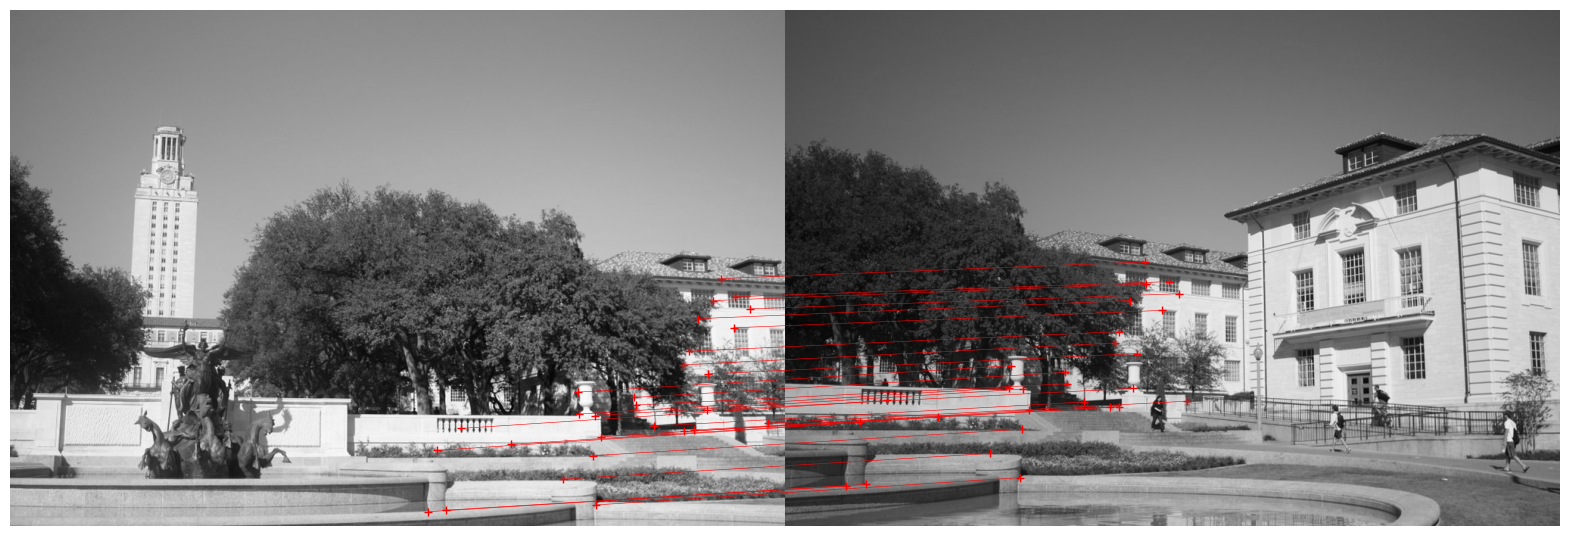
\includegraphics[width=0.90\linewidth]{student_response/figures/part1_inlier_pixel_cropped.png}
\caption{Inlier correspondences for the normalized pixel-patch descriptor (inlier ratio~0.28).
Accepted matches cluster near the strongest overlap zone and provide limited
spatial diversity for homography estimation.  The model is geometrically valid
but weakly constrained.}
\label{fig:part1_pixel_inliers}
\end{figure}

\begin{figure}[htbp]
\centering
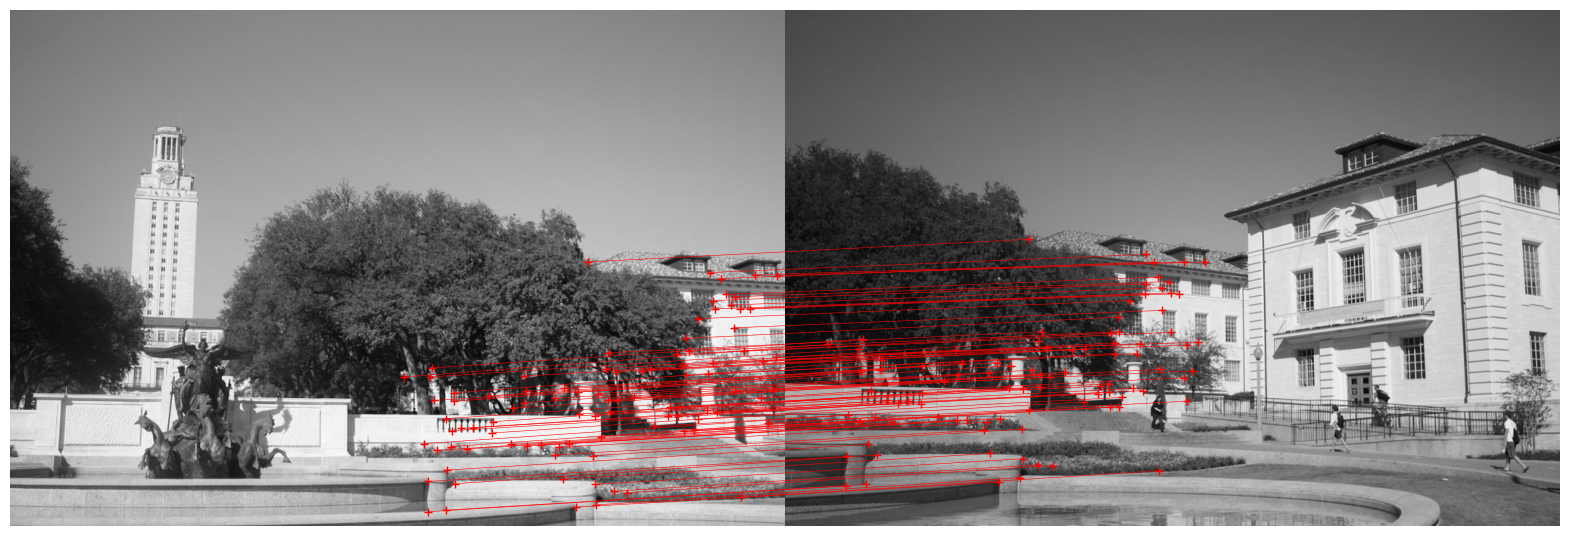
\includegraphics[width=0.90\linewidth]{student_response/figures/part1_inlier_hynet_cropped.png}
\caption{Inlier correspondences for HyNet (inlier ratio~0.94).
The matches span the building facade, trees, lower foreground, and distant
features---a much broader spatial support.  This wide coverage is why the HyNet
homography is better constrained, even though the per-inlier RMS residual is
slightly larger.}
\label{fig:part1_hynet_inliers}
\end{figure}

\begin{figure}[htbp]
\centering
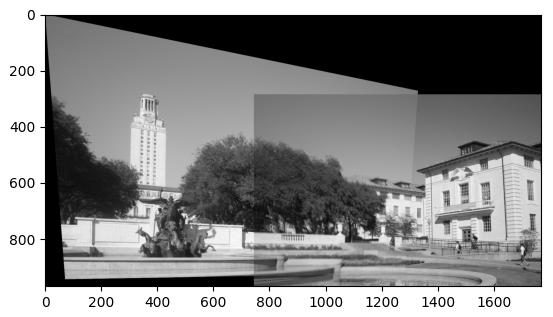
\includegraphics[width=0.86\linewidth]{student_response/figures/part1_stitched_pixel_cropped.png}
\caption{Panorama from the pixel-patch descriptor.  Alignment is geometrically
valid, but the smaller, spatially concentrated consensus set leaves the
homography with less distributional coverage across the full overlap region.}
\label{fig:part1_pixel_panorama}
\end{figure}

\begin{figure}[htbp]
\centering
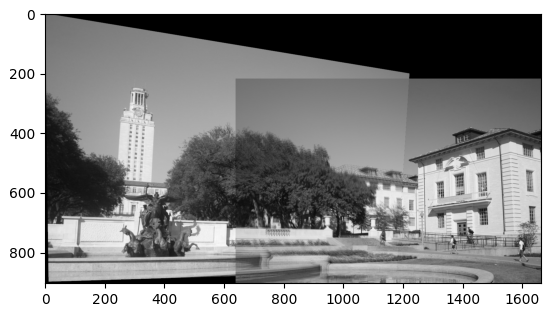
\includegraphics[width=0.86\linewidth]{student_response/figures/part1_stitched_hynet_cropped.png}
\caption{Panorama from HyNet correspondences.  The 94-inlier refit produces a
homography with strong distributional support across the entire overlap zone,
yielding more coherent structural alignment despite the higher per-inlier residual.}
\label{fig:part1_hynet_panorama}
\end{figure}

\subsection*{Part 1 Discussion}

The central lesson is that descriptor quality should not be evaluated by
conditional residual alone.  The pixel descriptor's lower RMS of 2.94~px is
meaningful only \emph{given} that a match was accepted; it says nothing about the
72\% of candidates it discarded.  For homography estimation the statistic that
matters is coverage: how well the accepted inliers span the image plane so that
all 8 homography degrees of freedom are well constrained.

HyNet earns its higher residual honestly.  Its learned representation is trained
to be invariant to local photometric change, mild geometric deformation, and
moderate viewpoint shift---precisely the conditions that cause raw-intensity
comparison to fail.  By tolerating a larger nominal distance between matched
descriptors, HyNet accepts correspondences from textured but photometrically
variable regions.  Those correspondences carry more spatial information for the
global model.  The remaining artifacts (seam visibility, black canvas regions)
reflect the simplified compositing strategy, not the geometric alignment quality.

\reporttakeaway{HyNet produces a much stronger geometric case: 94 inliers vs.\ 28,
broader spatial coverage, and a more coherent panorama.  The higher recall is more
valuable for homography estimation than the lower conditional residual of the pixel
descriptor.}

\subsection*{Limitations and Failure Modes}
The main failure mode is model mismatch: a single homography is exact only for
planar scenes or pure rotational camera motion.  The tower background contains
moderate depth variation, so residual parallax causes local misalignment that no
projective model can remove.  Additionally, the current compositing strategy does
not include exposure normalization or seam optimization.  If this were extended,
the most natural improvements would be mutual-nearest-neighbor plus ratio filtering,
normalized DLT (coordinate isotropic scaling), and seam-aware blending.

\clearpage
\section*{Part 2: Shape from Shading / Photometric Stereo}

\subsection*{Problem Setting and Pipeline Overview}
Part~2 recovers albedo and 3-D surface shape from the Yale-B face dataset.
Rather than single-image shape-from-shading (which is severely underconstrained),
the dataset provides 64 images of the same face under \emph{known}, varied
illumination with the camera fixed, enabling photometric stereo.  I implement
the reconstruction pipeline as follows:
(1) \emph{Ambient subtraction, clamping, and global normalization.}
(2) \emph{Vectorized least-squares photometric stereo} for all $P = 32\,256$
pixels simultaneously.
(3) \emph{Albedo and normal recovery} from the solved pseudonormal vectors.
(4) \emph{Gradient-field construction} from the recovered normals.
(5) \emph{Surface integration} via four required methods.

\subsection*{Theoretical Background}

Under the Lambertian model with orthographic projection, observed intensity at
pixel $(x,y)$ under illumination $i$ is:
\begin{equation}
  I_i(x,y) = \rho(x,y)\,\mathbf{l}_i^\top \mathbf{n}(x,y),
  \label{eq:lambertian}
\end{equation}
where $\rho(x,y)$ is surface albedo, $\mathbf{n}(x,y)$ is the unit inward
normal, and $\mathbf{l}_i \in \mathbb{R}^3$ is the known unit light direction.
Defining the \emph{pseudonormal} $\mathbf{g} = \rho\mathbf{n}$ linearizes
Eq.~\eqref{eq:lambertian}:
\begin{equation}
  \mathbf{i}(x,y) = \mathbf{L}\,\mathbf{g}(x,y),
  \quad
  \mathbf{L} \in \mathbb{R}^{64 \times 3},\;
  \mathbf{i}(x,y) \in \mathbb{R}^{64}.
  \label{eq:photometric_system}
\end{equation}
With $N = 64 \gg 3$, the system is robustly overdetermined and admits a stable
closed-form least-squares solution per pixel.  All pixels are solved simultaneously:
\begin{equation}
  \mathbf{G}^\star = \arg\min_{\mathbf{G}} \|\mathbf{L}\mathbf{G} - \mathbf{I}\|_F^2,
  \qquad \mathbf{I} \in \mathbb{R}^{64 \times P},\; \mathbf{G} \in \mathbb{R}^{3 \times P}.
  \label{eq:batch_lstsq}
\end{equation}
Albedo and normal are then recovered as:
\begin{equation}
  \rho = \|\mathbf{g}\|_2, \qquad
  \mathbf{n} = \frac{\mathbf{g}}{\|\mathbf{g}\|_2 + \varepsilon}.
  \label{eq:albedo_normal}
\end{equation}

For a height field $z(x,y)$ under orthographic projection, the surface normal is
proportional to $[-p\;-q\;1]^\top$, where $p = \partial z/\partial x$ and
$q = \partial z/\partial y$.  Inverting this relation gives the discrete gradient
field:
\begin{equation}
  p = -\frac{n_x}{n_z}, \qquad q = -\frac{n_y}{n_z}.
  \label{eq:gradient_field}
\end{equation}
An ideal Lambertian surface satisfies the integrability condition
$\partial p/\partial y = \partial q/\partial x$.  Real data violates this due to
shadows, specularities, and model mismatch, so the integration path matters.

\textbf{Preprocessing.}
\begin{equation}
  I_i^+(x,y) = \max\!\left(I_i(x,y) - I_{\mathrm{amb}}(x,y),\;0\right),
  \quad
  \hat{I}_i(x,y) = \frac{I_i^+(x,y)}{\max_{j,u,v} I_j^+(u,v)}.
  \label{eq:preprocess}
\end{equation}
Ambient subtraction removes the constant non-directional component; clamping
prevents the least-squares system from modeling physically impossible negative
intensities; global (not per-image) normalization preserves relative intensity
relationships across all 64 lighting directions.

\textbf{Integration methods.}

\emph{Row first:}
$\displaystyle z_{\mathrm{row}}(r,c)
  = \sum_{j=0}^{c-1} p(0,j) + \sum_{i=0}^{r-1} q(i,c).$

\emph{Column first:}
$\displaystyle z_{\mathrm{col}}(r,c)
  = \sum_{i=0}^{r-1} q(i,0) + \sum_{j=0}^{c-1} p(r,j).$

\emph{Average:} $z_{\mathrm{avg}} = \tfrac{1}{2}(z_{\mathrm{row}} + z_{\mathrm{col}})$.

\emph{Random path:}
$\displaystyle z_{\mathrm{rand}}(r,c)
  = \frac{1}{K}\sum_{k=1}^{K}\sum_{(u,v)\in\mathcal{P}_k(r,c)} \Delta z(u,v),$
where each $\mathcal{P}_k$ is a uniformly sampled monotone path from $(0,0)$
to $(r,c)$ with $K = 20$.

\subsection*{Implementation Choices and Technical Discussion}

\textbf{Global normalization.}  Per-image normalization would distort relative
illumination intensities and make the linear system~\eqref{eq:photometric_system}
inconsistent.  Using a single global maximum preserves the physical photometric
relationship across all 64 observations.

\textbf{Vectorized least squares.}  Reshaping the $N \times h \times w$ image
stack to $N \times P$ and calling \texttt{torch.linalg.lstsq} once solves all
pixels in a single batched LAPACK call.  This is orders of magnitude faster than
iterating over $P = 32\,256$ pixels.

\textbf{Stable gradient conversion.}  Dark pixels and tangent-grazing normals
can have $|n_z| \approx 0$; dividing by $n_z$ directly would produce numerical
explosions.  An elementwise safeguard limits these outliers without affecting
well-lit frontal regions.

\textbf{Random-path reproducibility.}  The random-path integrator uses a fixed
PyTorch seed (0) for reproducibility despite stochastic sampling.

\subsection*{Single-Subject Integration Comparison on \texttt{yaleB01}}

\begin{figure}[htbp]
\centering
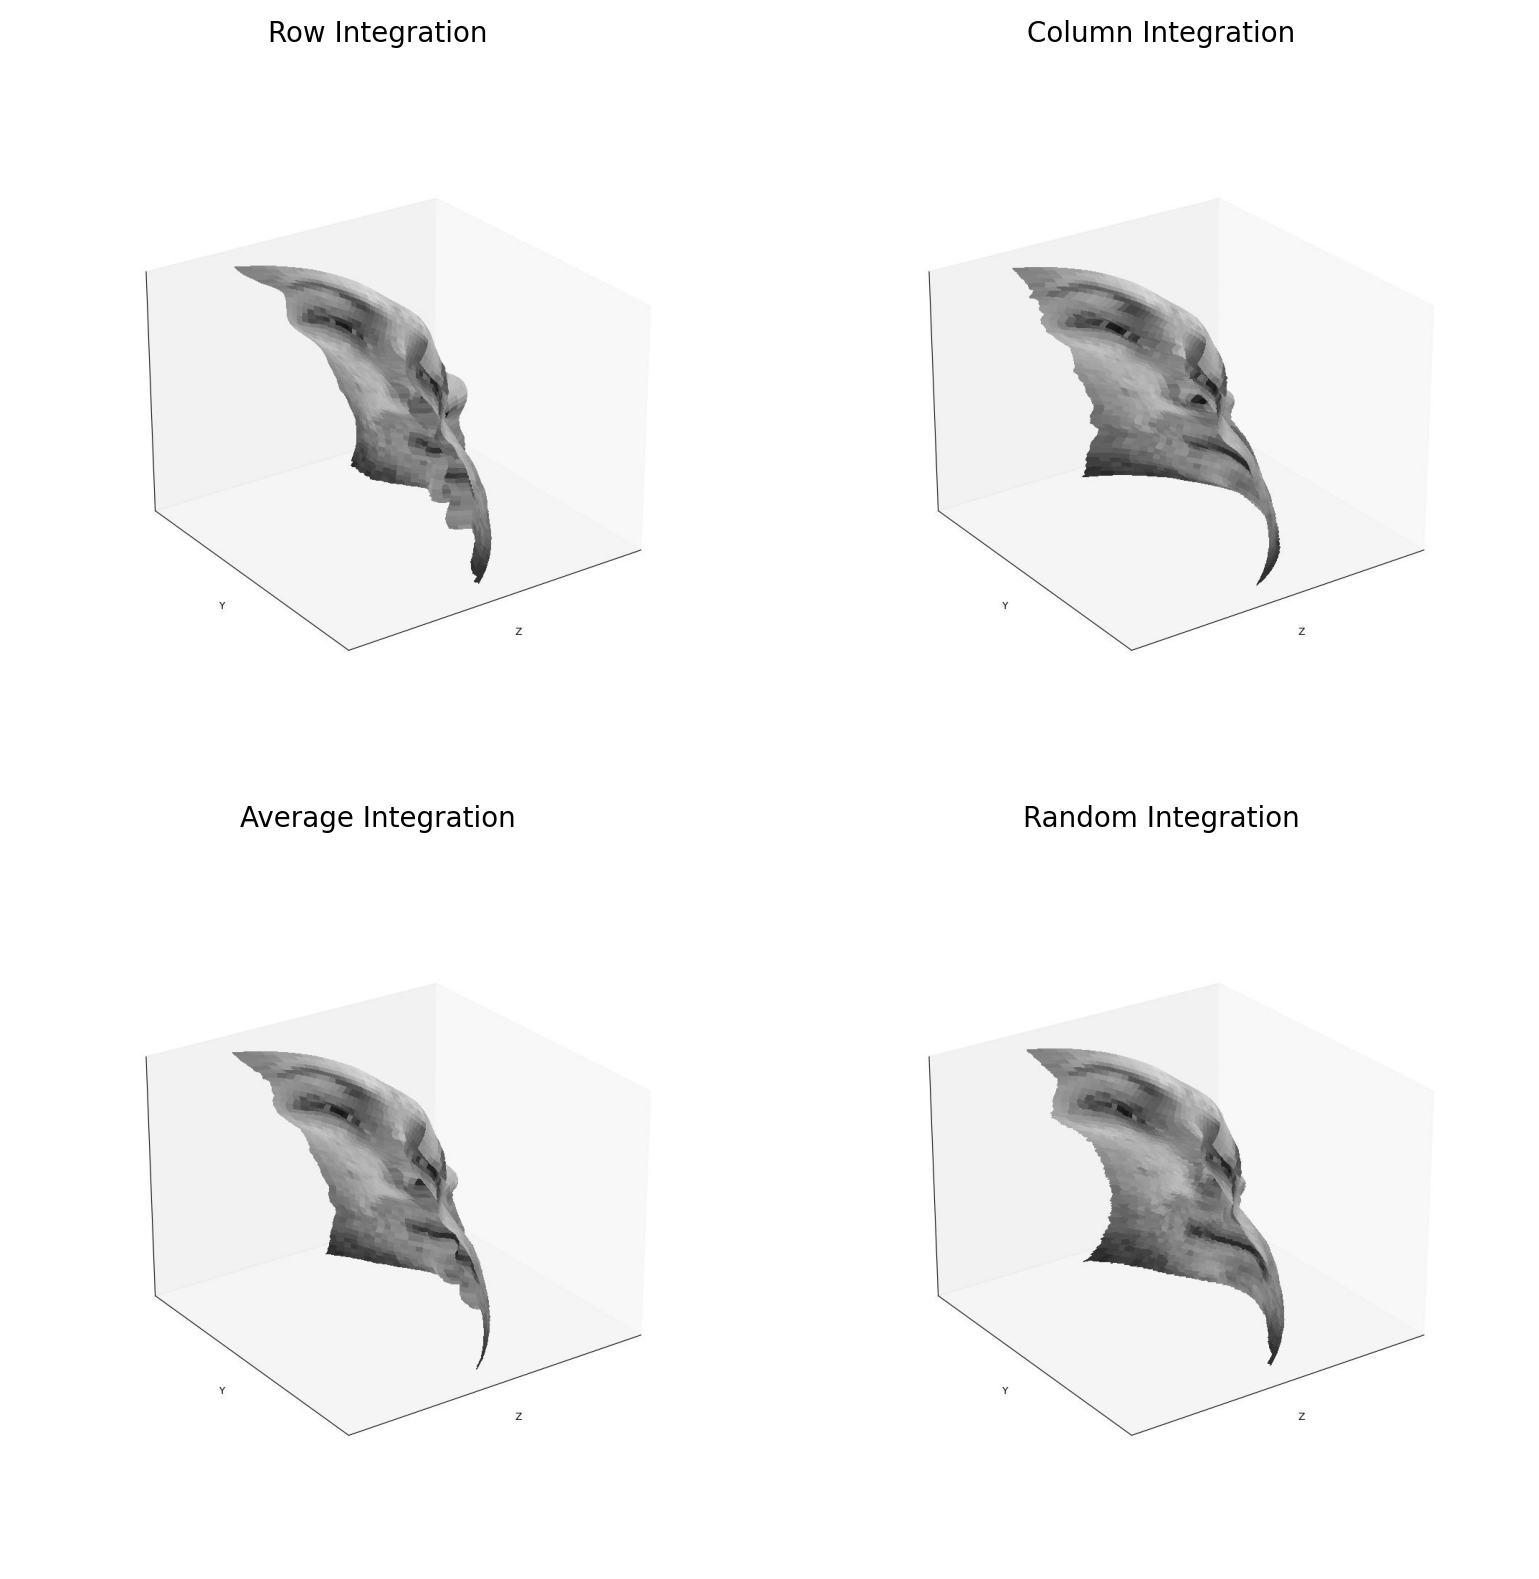
\includegraphics[width=0.95\linewidth]{student_response/figures/yaleB01_method_compare.png}
\caption{Height maps for \texttt{yaleB01} under the four required integration
methods.  Row-first and column-first each inherit a visible directional bias from
the primary accumulation axis.  Averaging the two largely cancels this bias.
Random-path integration is marginally smoother but not substantially different
from the average method.}
\label{fig:part2_method_compare}
\end{figure}

\begin{table}[htbp]
\centering
\small
\begin{tabular}{l|c|c|c|c|c}
\hline
Method & Runtime (s) & Height std. & Height range & Mean grad.\ mag. & Centered RMSE to avg. \\
\hline
Row     & 3.004 & 18.9004 & 103.0051 & 0.7203 & 3.7403 \\
Column  & 2.653 & 20.9398 & 109.5881 & 0.7659 & 3.7403 \\
Average & 2.658 & 19.5924 & 105.6616 & 0.6786 & 0.0000 \\
Random  & 79.461 & 17.4720 & 90.6959  & 0.7260 & 5.2158 \\
\hline
\end{tabular}
\caption{Integration-method comparison for \texttt{yaleB01}.
Height statistics are relative (not metric).
`Centered RMSE to avg.' compares each method against the average surface after
subtracting the global depth offset.
Note that row and column produce identical centered RMSE by
construction: $z_{\mathrm{avg}} = \tfrac{1}{2}(z_{\mathrm{row}}+z_{\mathrm{col}})$,
so they are symmetric deviations.
The random method runs $29.9\times$ slower than the average method while
producing a larger centered RMSE.}
\label{tab:part2_method_metrics}
\end{table}

Table~\ref{tab:part2_method_metrics} reveals several non-obvious results.  The
row and column methods produce centered RMSE values of exactly 3.7403, which
follows algebraically from the averaging definition.  The average method reduces
the mean gradient magnitude from $\approx 0.72$--0.77 (directional methods) to
0.679, consistent with a less-biased, smoother surface.

The random-path method produces a \emph{larger} centered RMSE than either
directional method (5.22 vs.\ 3.74), indicating that 20 sampled paths per pixel
still introduce path-dependent noise.  The total number of monotone paths from
$(0,0)$ to $(r,c)$ is $\binom{r+c}{r}$, which reaches $\sim 10^{50}$ near the
image center.  With $K = 20$ paths, the stochastic estimator has high variance
and does not converge; it introduces its own noise rather than averaging it away.
The average method implicitly computes a deterministic two-path average---a much
lower-variance estimator in this setting.  Combined with its $29.9\times$ runtime
penalty, random-path integration is not cost-effective here.

\subsection*{Recovered Albedo and Surface Normals}

\begin{figure}[htbp]
\centering
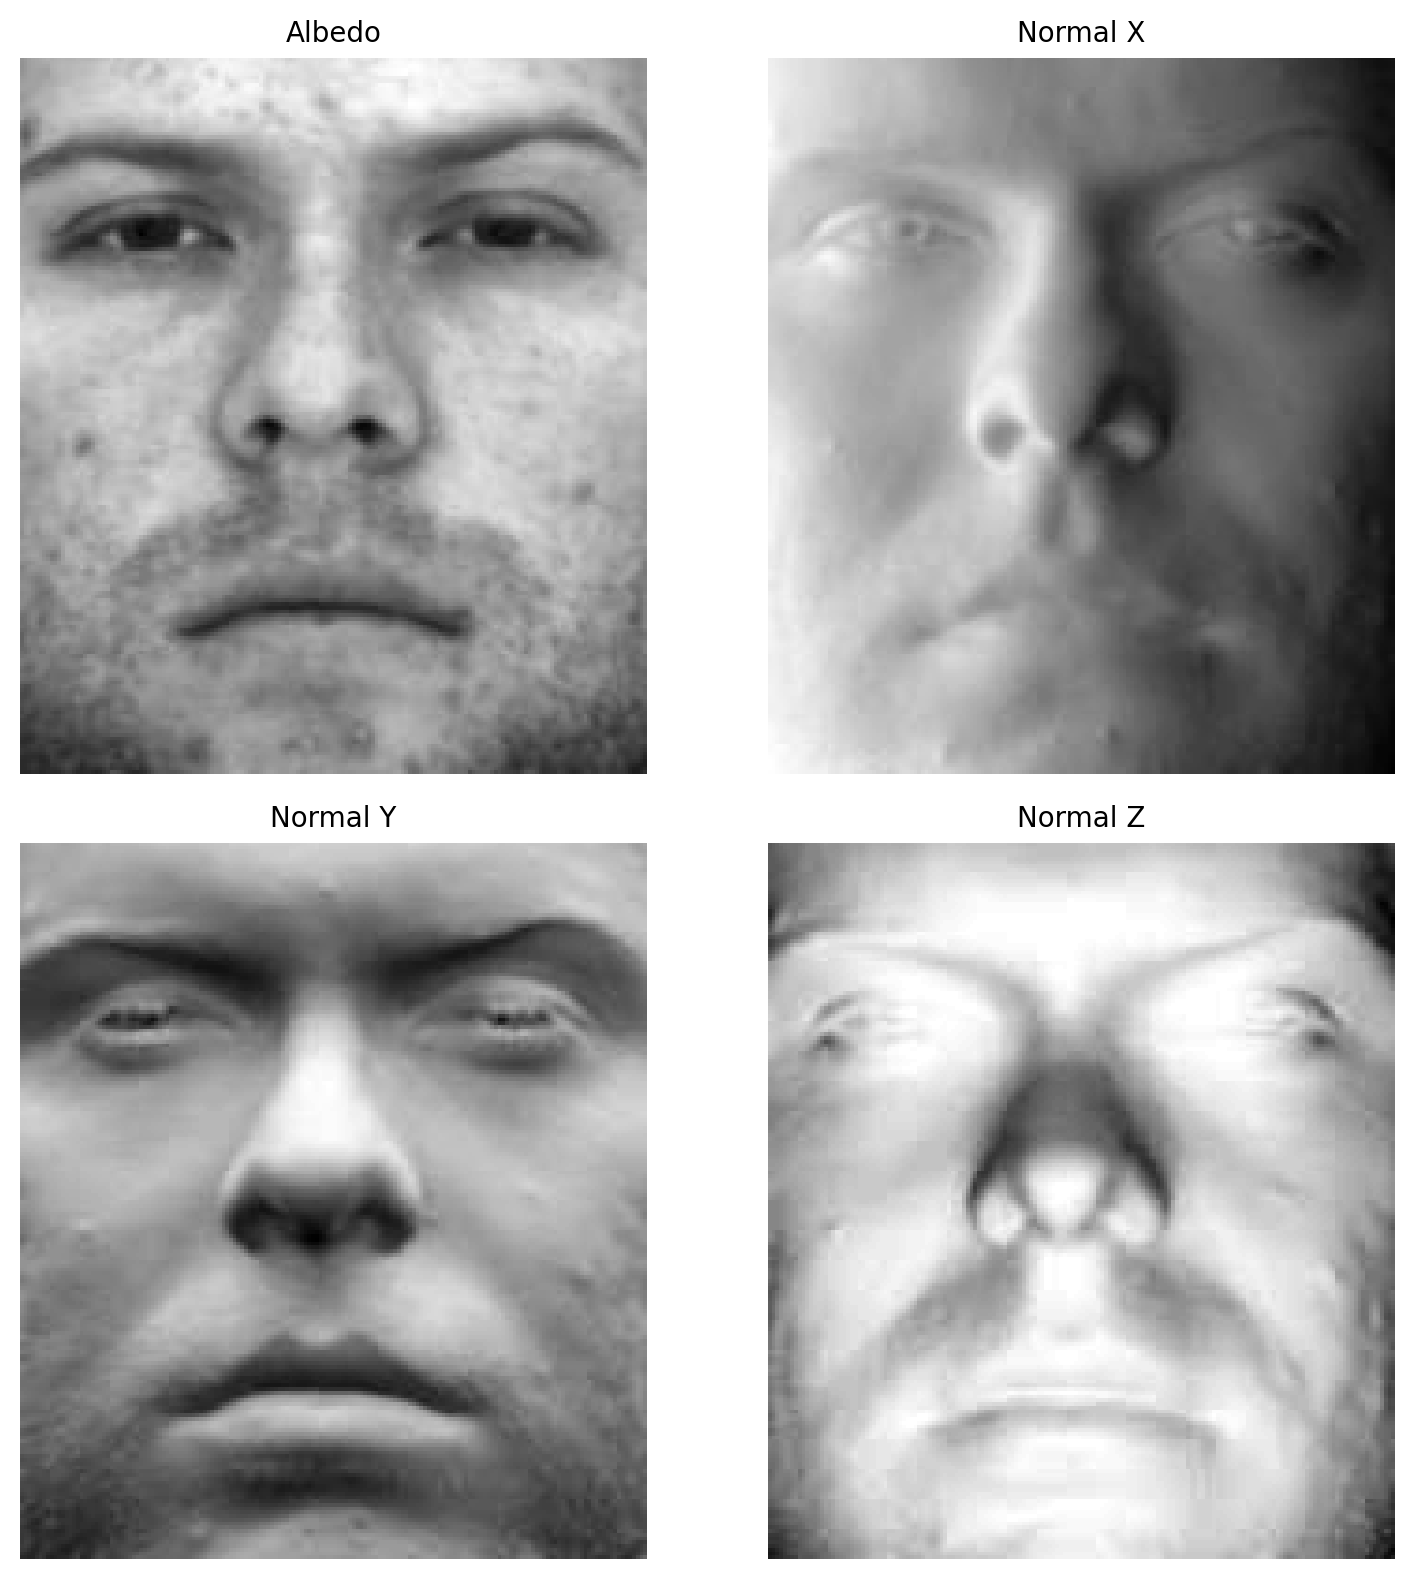
\includegraphics[width=0.93\linewidth]{student_response/figures/yaleB01_normals_grid.png}
\caption{Recovered albedo and surface-normal components for \texttt{yaleB01}.
The albedo captures coarse reflectance structure.
$n_x$ changes monotonically across the nose and cheeks; $n_y$ changes between
forehead, nose tip, and chin; $n_z$ remains bright over the central face,
confirming that the frontal surface is predominantly camera-facing.
Noise appears near hair and shadow boundaries where the Lambertian model breaks down.}
\label{fig:part2_normals}
\end{figure}

The normal component maps serve as an internal validity check on the
photometric-stereo solve before integration is discussed.
If the least-squares stage had failed, the maps would appear unstructured or
dominated by noise.  The structured gradients in Figure~\ref{fig:part2_normals}
confirm that the overdetermined system captures physically meaningful orientation
information despite partial Lambertian assumption violations.

\subsection*{Multi-Subject Analysis}

\begin{figure}[htbp]
\centering
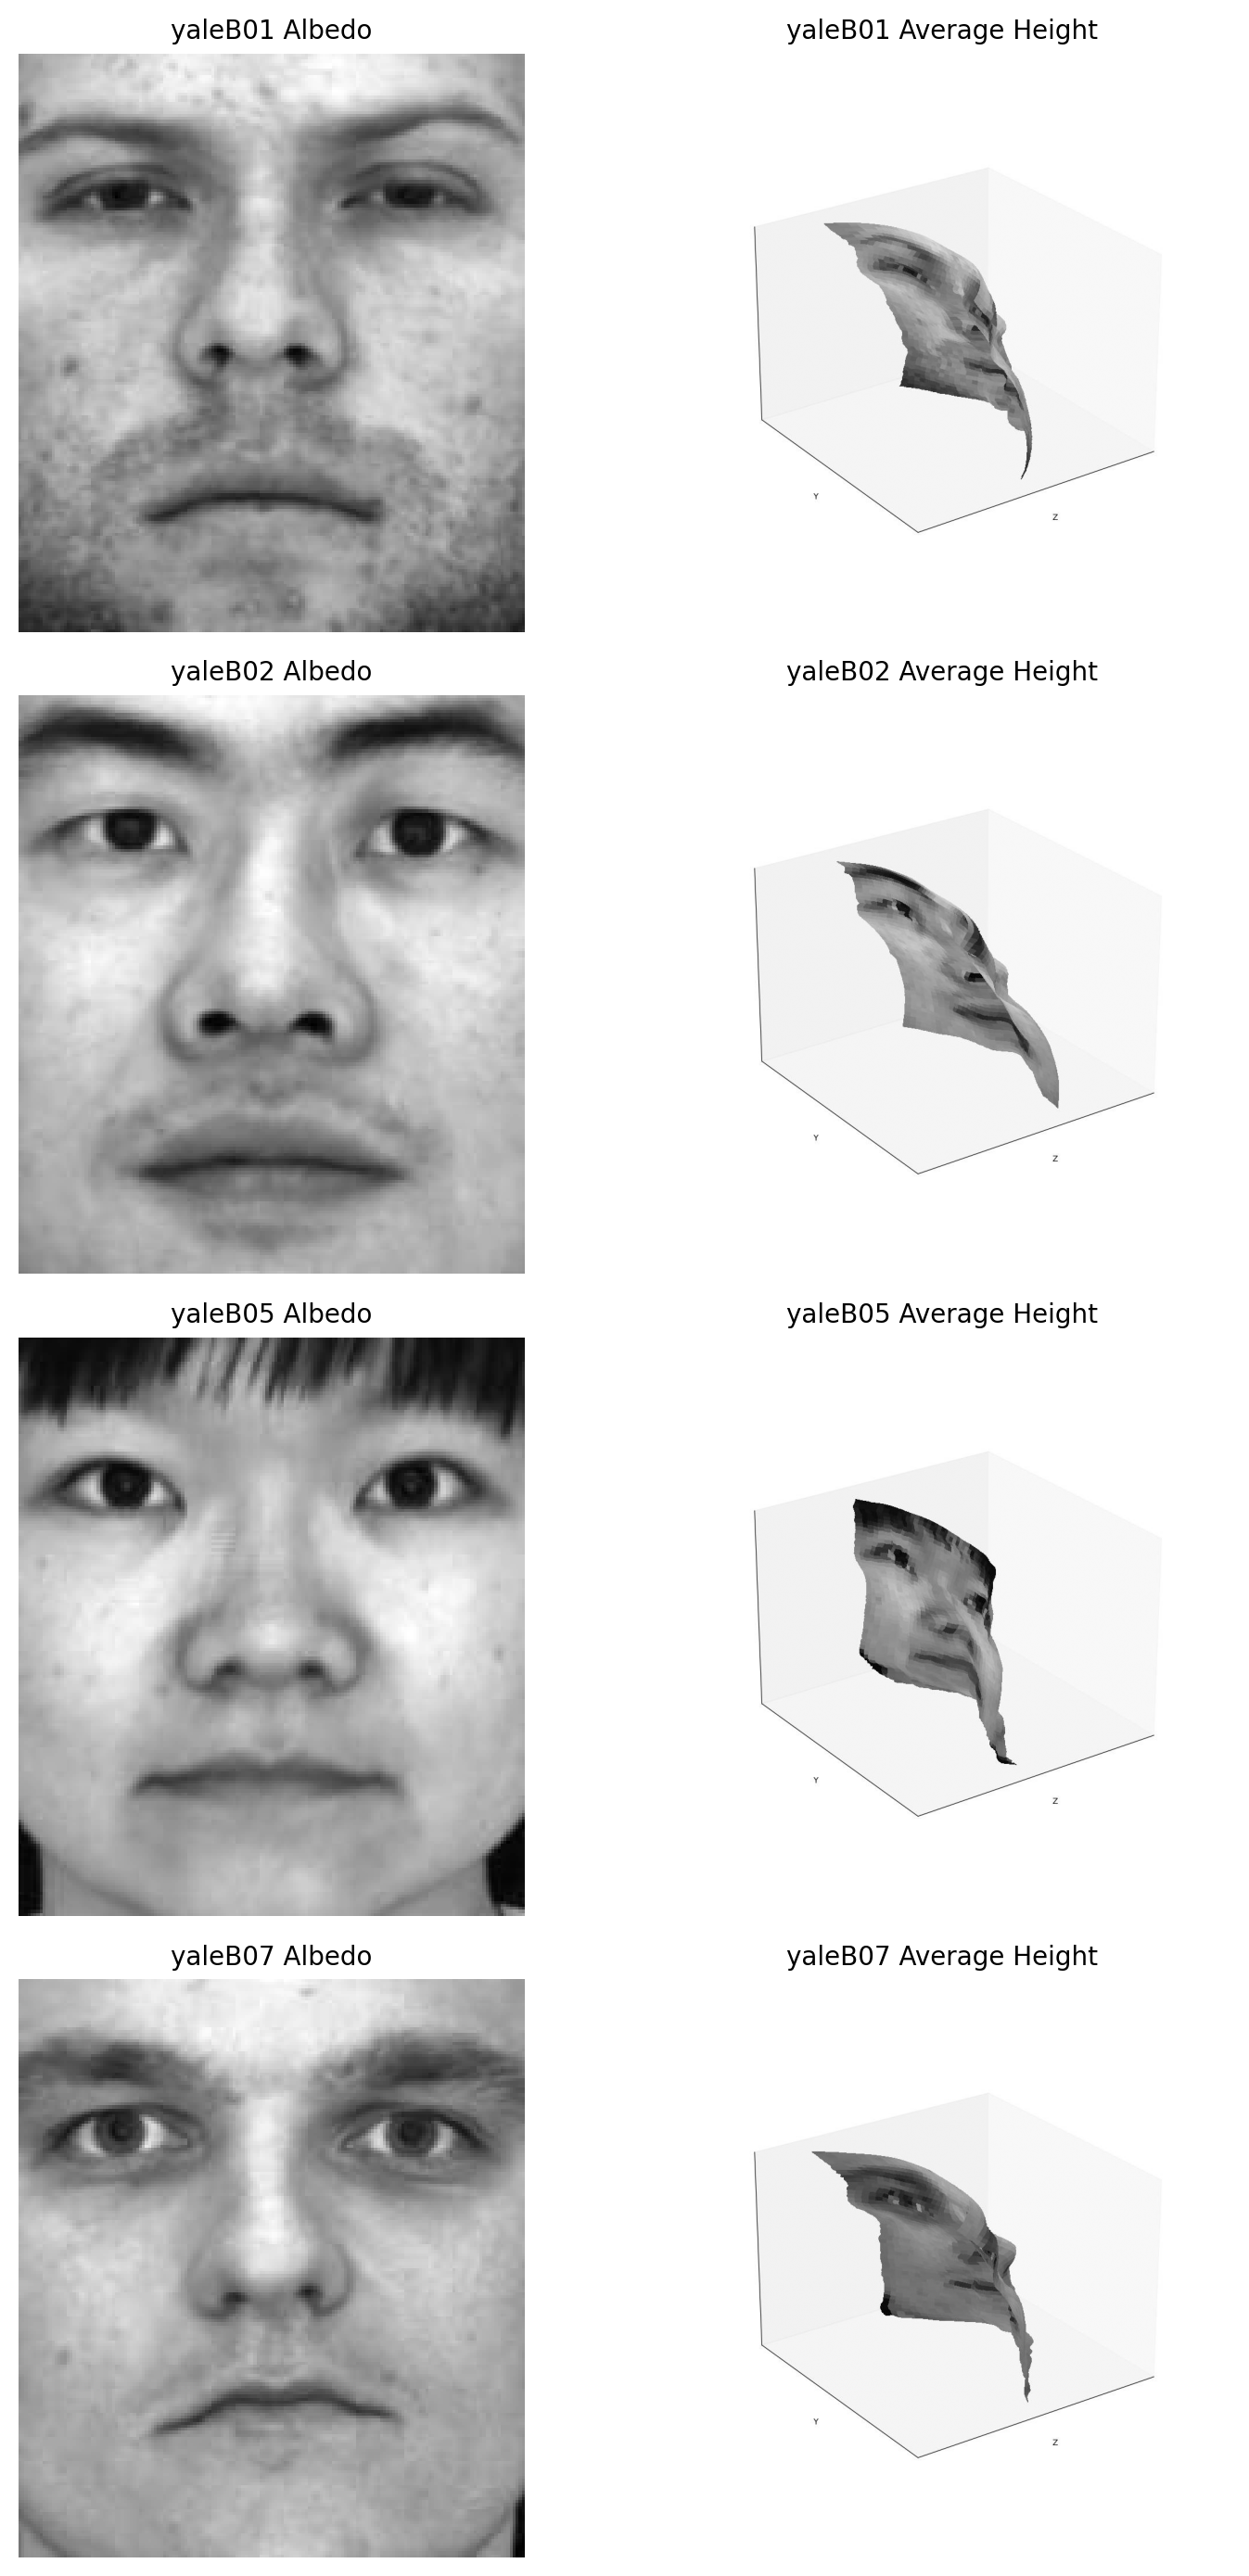
\includegraphics[height=0.74\textheight,keepaspectratio]{student_response/figures/all_subjects_average_results.png}
\caption{Average-integration results for all four required Yale subjects.
The dominant facial structure is recovered consistently.  Reconstruction quality
degrades most clearly at hairlines, cast-shadow boundaries, and background pixels,
which violate the Lambertian smooth-surface model most severely.}
\label{fig:part2_all_subjects}
\end{figure}

\begin{table}[htbp]
\centering
\small
\begin{tabular}{l|c|c|c|c|c|c}
\hline
Subject & Albedo mean & Albedo std. & Mean $n_z$ & Std.\ $n_z$ & Integrability MAE & Height range \\
\hline
\texttt{yaleB01} & 0.5317 & 0.1397 & 0.8397 & 0.1200 & 0.0229 & 105.6616 \\
\texttt{yaleB02} & 0.5331 & 0.1507 & 0.8781 & 0.1047 & 0.0166 & 109.0149 \\
\texttt{yaleB05} & 0.4702 & 0.1696 & 0.8885 & 0.1125 & 0.0253 & 64.6000 \\
\texttt{yaleB07} & 0.4408 & 0.1112 & 0.8111 & 0.1311 & 0.0254 & 125.8820 \\
\hline
\end{tabular}
\caption{Subject-level diagnostics (average integration).
Integrability MAE measures the mean absolute violation of
$\partial p/\partial y = \partial q/\partial x$ and is the most direct indicator of
gradient-field quality: lower is better.
\texttt{yaleB02} achieves the lowest value (0.0166); \texttt{yaleB05} the smallest
height range, consistent with hair-induced photometric signal reduction.
All four subjects fall in the narrow integrability band $[0.017, 0.025]$,
confirming that the same systematic model violations affect the entire dataset.}
\label{tab:part2_subject_metrics}
\end{table}

Three cross-subject observations stand out.
\texttt{yaleB05} has the smallest height range (64.6 vs.\ 90--126 for others),
likely due to hair-over-forehead occlusion reducing the effective photometric
signal.  \texttt{yaleB07} has the largest height range (125.9) and lowest mean
$n_z$ (0.811), indicating stronger facial relief and more oblique average
normals.  The narrow integrability MAE band across all subjects suggests that
the violated assumptions (cast shadows, hair, background) are dataset-level
properties, not per-subject outliers.

\subsection*{Lambertian Assumption Violations}

\begin{figure}[htbp]
\centering
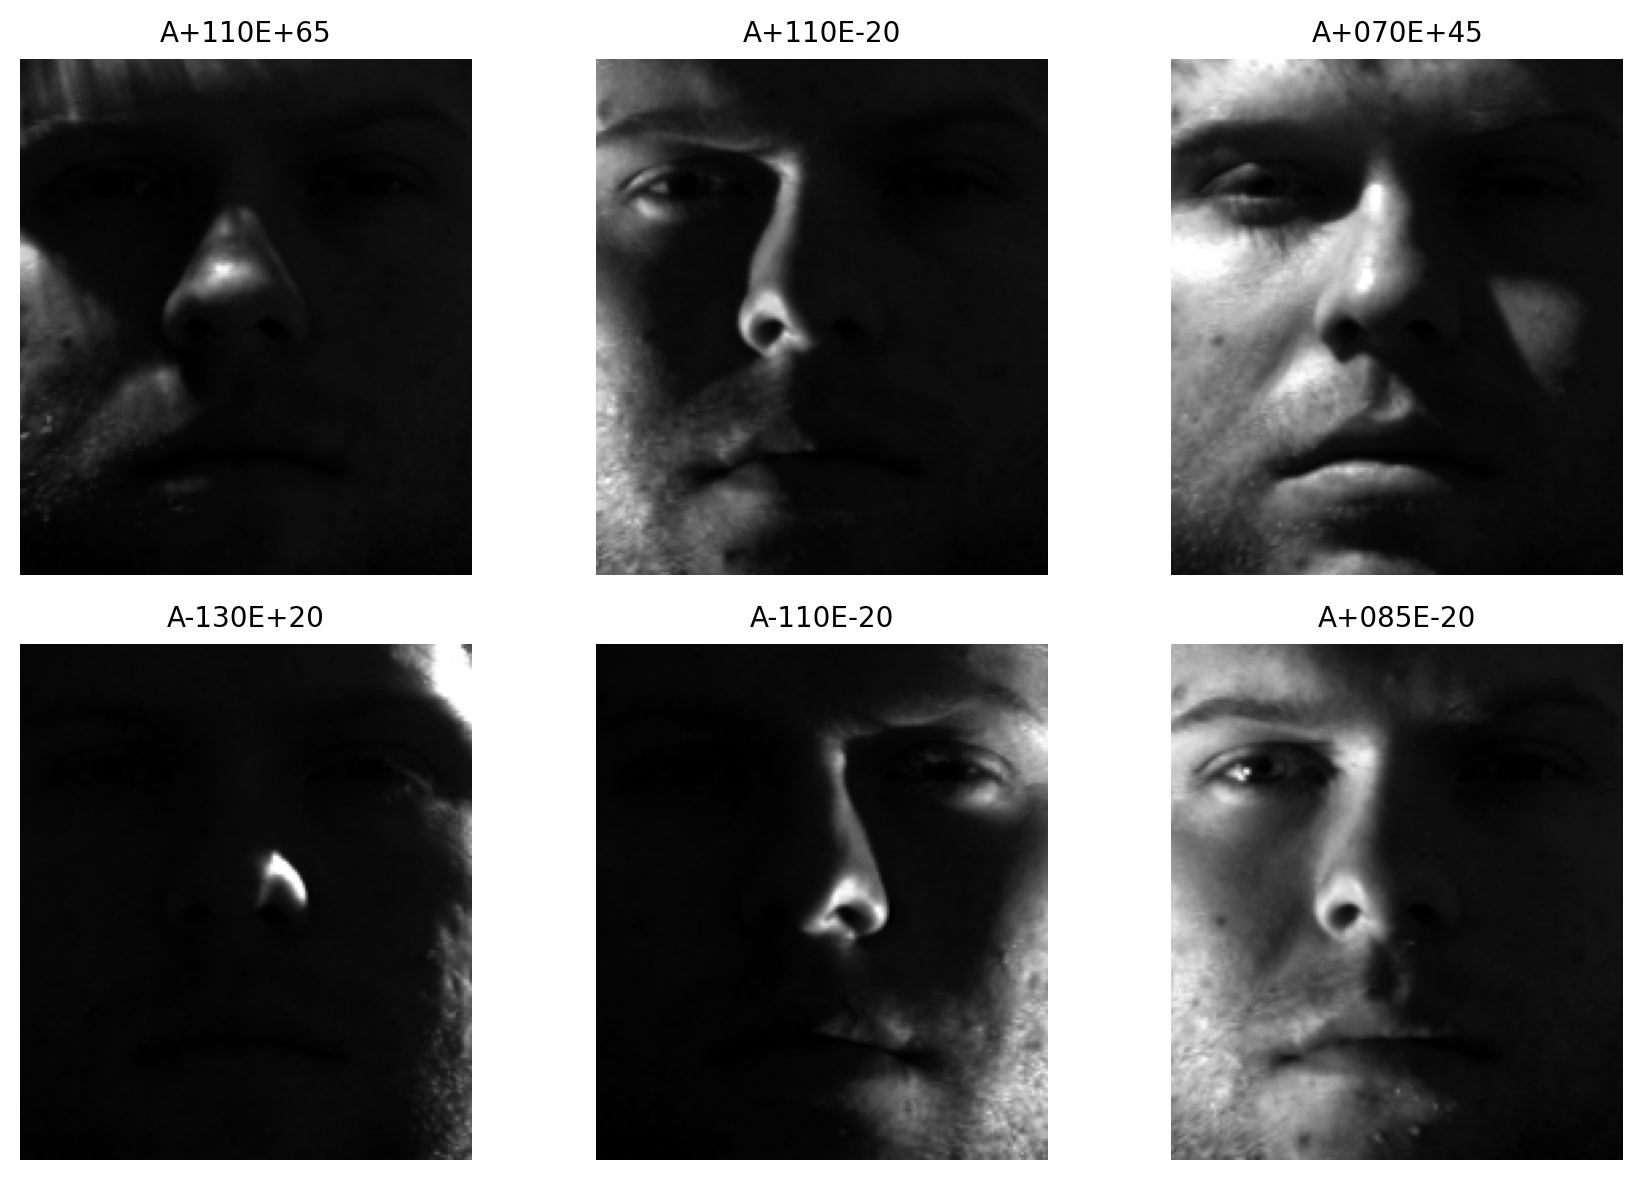
\includegraphics[width=0.92\linewidth]{student_response/figures/yaleB01_assumption_inputs.png}
\caption{Representative \texttt{yaleB01} input images illustrating why the Yale-B
data is not an ideal Lambertian benchmark.  From near-frontal to extreme
side-illumination: cast shadows, hair, near-saturation at highlights, and deep
self-shadow regions are all visible.
Each violation disturbs the linear image-formation model and degrades the quality
of the recovered normals and height map.}
\label{fig:part2_assumptions}
\end{figure}

The Yale-B images violate the Lambertian model in at least five distinct ways.
\emph{(1) Cast and attached shadows.}  At extreme illumination angles, large
face regions fall in shadow, producing near-zero intensities where the model
predicts a positive cosine response.  This biases the least-squares estimate
toward smaller $\|\mathbf{g}\|$, compressing albedo and potentially skewing
the normal direction.
\emph{(2) Non-Lambertian reflectance.}  Skin has a specular component; hair is
essentially non-Lambertian.  Both add structured residuals to the least-squares
system.
\emph{(3) Background contamination.}  Background pixels belong to a different
geometry from the facial surface; their recovered normals are meaningless and
contribute noise near the crop boundary.
\emph{(4) Interreflections.}  Concave facial regions (eye sockets, under the
nose) receive indirect illumination not modeled by the single-bounce Lambertian
equation.
\emph{(5) Expression and alignment micro-variation.}  Slight expression changes
or positioning shifts across 64 captures introduce spatial inconsistencies in the
normal field.

\subsection*{Subset-of-Viewpoints Experiment}

\begin{figure}[htbp]
\centering
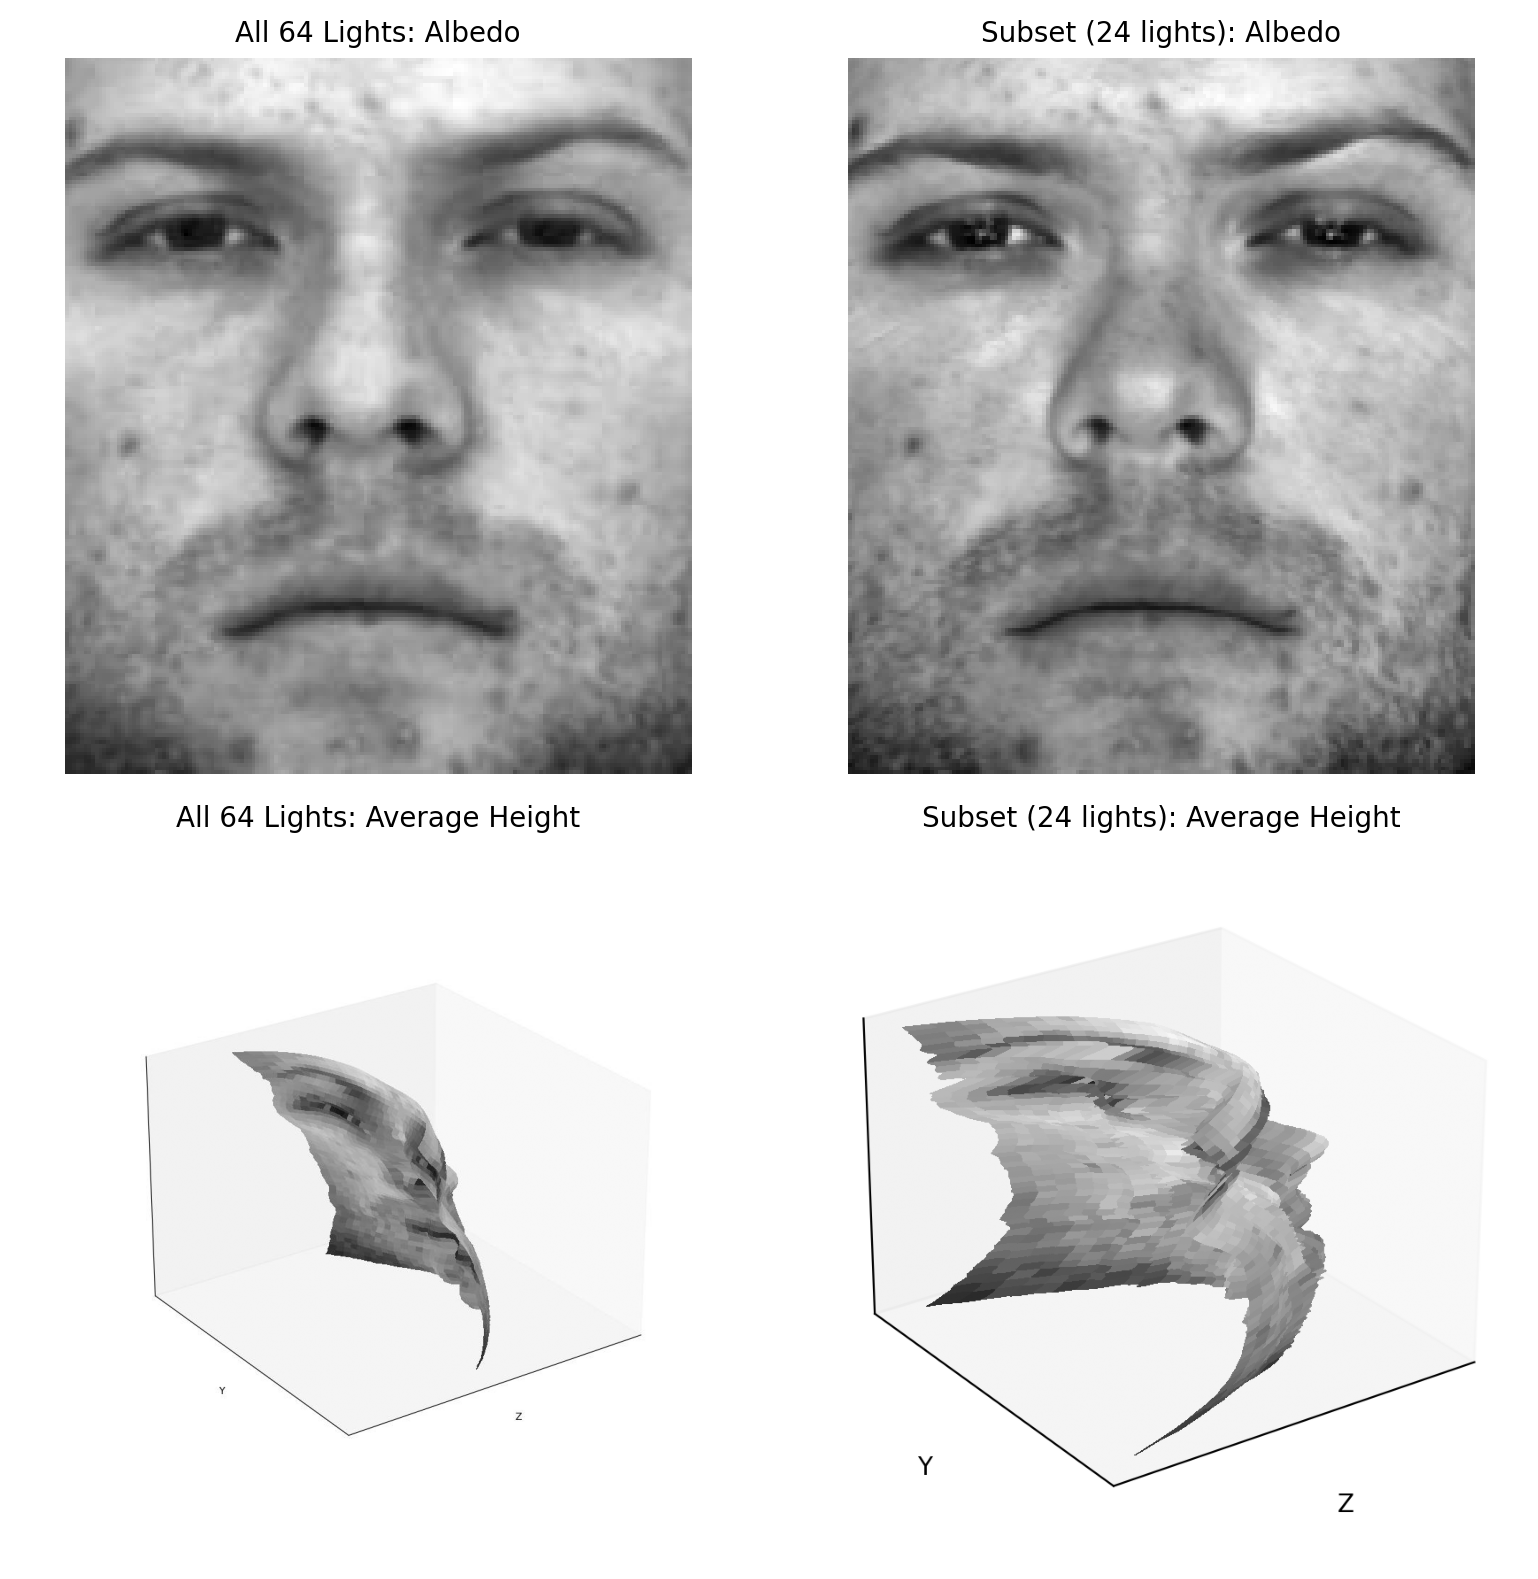
\includegraphics[width=0.95\linewidth]{student_response/figures/yaleB01_subset_compare.png}
\caption{All-64-image vs.\ 24-image moderate-lighting subset
($|\mathrm{azimuth}| \le 35^\circ$, $|\mathrm{elevation}| \le 35^\circ$) for
\texttt{yaleB01}.  The subset reduces the most extreme shadows but produces a
more blocky and less stable height map because the lighting matrix becomes
poorly conditioned.}
\label{fig:part2_subset_compare}
\end{figure}

\begin{table}[htbp]
\centering
\small
\begin{tabular}{l|c|c|c|c|l}
\hline
Lighting set & \# Images & Cond.\ number & $\sigma_{\min}$ & $\sigma_{\max}$ & Qualitative result \\
\hline
All lights      & 64 & 1.4593 & 3.5822 & 5.2277 & Best overall reconstruction \\
Moderate subset & 24 & 3.5228 & 1.2730 & 4.4847 & Less stable, more blocky depth \\
\hline
\end{tabular}
\caption{Lighting-matrix conditioning for the subset experiment on \texttt{yaleB01}.
The condition number of $\mathbf{L}$ more than doubles (1.46 to 3.52) and
$\sigma_{\min}$ drops from 3.58 to 1.27 when restricted to 24 moderate directions.
Geometrically, the 24 directions are concentrated in a narrow cone, so normals
pointing toward the face periphery are poorly constrained.}
\label{tab:part2_subset}
\end{table}

The subset experiment isolates an important design principle: conditioning quality
and assumption quality are in tension.  Removing extreme azimuth/elevation images
reduces cast shadows and specular highlights, but also concentrates $\mathbf{L}$
in direction space.  The condition number more than doubles and $\sigma_{\min}$
drops by 64\%, making the system far less informative for recovering oblique
normals.  The result is a flatter, more blocky height map.  In this dataset,
broader illumination coverage outweighs the cost of including shadow-affected images.

\subsection*{Computation and Performance Summary}

\begin{table}[htbp]
\centering
\small
\begin{tabular}{l|l|c|l}
\hline
Experiment & Workload proxy & Runtime (s) & Main computational driver \\
\hline
Part 1 pixel  & 100 matches, 30k RANSAC, 225-D & 20.211 & Exhaustive matching + RANSAC \\
Part 1 HyNet  & 100 matches, 30k RANSAC, 128-D & 20.164 & HyNet encoding + RANSAC \\
Part 2 row    & 64 images, 32\,256 pixels & 3.004  & Vectorized least squares \\
Part 2 column & 64 images, 32\,256 pixels & 2.653  & Vectorized least squares \\
Part 2 average & 64 images, 32\,256 pixels & 2.658 & Vectorized least squares \\
Part 2 random & 64 images, 32\,256 pixels, 20 paths & 79.461 & Stochastic path integration \\
\hline
\end{tabular}
\caption{End-to-end runtime profile.  Part~1 timings are dominated by the
30\,000-iteration RANSAC loop; descriptor encoding has minimal overhead (hence
the near-identical pixel vs.\ HyNet times).
Part~2 deterministic methods are fast because the entire photometric solve is a
single batched LAPACK call.  Only random-path integration breaks linear scaling
because it iterates over $h \times w \times 20 = 645\,120$ stochastic paths in
Python.}
\label{tab:runtime_profile}
\end{table}

\subsection*{Part 2 Discussion}

The best overall integration method is \texttt{average}.  Mathematically,
$z_{\mathrm{avg}} = \tfrac{1}{2}(z_{\mathrm{row}} + z_{\mathrm{col}})$;
if the noise in the two directional surfaces is symmetric and uncorrelated,
averaging reduces variance by $1/\sqrt{2}$ relative to either directional method.
Empirically, this cancellation is visible in Figure~\ref{fig:part2_method_compare}
and confirmed by the reduced mean gradient magnitude and lower height standard
deviation in Table~\ref{tab:part2_method_metrics}.

The random-path method is theoretically appealing but empirically disappointing
in this setting.  The problem is that $K = 20$ paths is far too few relative to
the $\binom{r+c}{r}$ total monotone paths available.  With high variance per
path and only 20 samples, the estimator introduces its own noise rather than
averaging it away---which is why its centered RMSE exceeds that of the simple
directional methods.  The average method implicitly computes a deterministic
two-path average, which is a much lower-variance estimator.

The multi-subject analysis confirms that reconstruction quality is stable across
all four subjects.  Integrability MAE remains within a factor of 1.5 across
subjects, indicating the pipeline is not brittle to individual subject variation.
Remaining artifacts reflect dataset-level assumption violations rather than
per-subject implementation failures.

\reporttakeaway{Reconstruction quality in photometric stereo is a system-level
property: lighting matrix conditioning, preprocessing fidelity, normal stability,
and integration bias all interact.  Among the four required methods,
\texttt{average} achieves the best balance: it reduces directional path bias,
runs at the cost of a single deterministic method, and generalizes consistently
across all four subjects.  The random-path method does not improve on this
despite a $29.9\times$ runtime increase.}

\subsection*{Limitations and Future Improvements}
The dominant failure modes come from reflectance-model mismatch.  Cast shadows,
hair, specular highlights, and background contamination inject structured
non-Lambertian residuals into the least-squares system.  A more robust pipeline
would use robust regression (e.g., iteratively reweighted least squares with
shadow masking) for the photometric-stereo solve, and Poisson-equation surface
integration to replace path-dependent methods.  Those extensions would improve
both normal quality and surface stability but lie beyond the scope of this
assignment.

\section*{Conclusion}

This assignment demonstrates two complementary principles in geometric computer
vision.

\textbf{Part~1.}  Descriptor quality should be measured holistically, not by a
single scalar.  The pixel-patch descriptor yields lower RMS inlier residual but
far fewer geometrically consistent correspondences.  HyNet yields higher residual
but 94\% inlier recall, producing a homography estimated from a $23.5\times$
overdetermined system with broad spatial coverage.  The resulting HyNet panorama
is qualitatively and geometrically stronger.

\textbf{Part~2.}  Surface reconstruction quality is a system-level property.
Lighting diversity (conditioning), preprocessing fidelity, normal estimation
stability, and integration bias all interact.  The subset experiment demonstrates
that removing assumption-violating images can hurt more than it helps when it
also reduces directional coverage.  Among the four required integration strategies,
averaging row-first and column-first is the most effective: it removes the dominant
directional bias at no additional cost and with lower variance than 20-path
random integration.

Both parts reveal the same underlying pattern: the best engineering solution is
not the most elaborate one, but the one that best balances model expressiveness,
measurement quality, and computational cost.

\reporttakeaway{HyNet is the stronger descriptor for this stitching task; average
integration is the strongest surface-recovery method for the Yale photometric-stereo
data.  In both cases the superiority follows from principled geometric reasoning,
not just empirical observation.}

\section*{AI Use Acknowledgment}
\textbf{AI Use Acknowledgment.} I used AI tools as a coding and writing assistant
for implementation cleanup, experiment automation, metric summarization, repository
packaging, and report drafting.  I reviewed and validated all code, outputs,
equations, figures, and interpretations before finalizing this submission.

\section*{Assignment Requirement Mapping}
\begin{itemize}
\item \textbf{Part 1 method and implementation details:} `Problem Setting',
  `Theoretical Background', `Mathematical Formulation', and `Implementation Choices'.
\item \textbf{Comparison between raw patch and HyNet:} Table~\ref{tab:part1_quant},
  Figures~\ref{fig:part1_pixel_inliers}--\ref{fig:part1_hynet_panorama}, and
  `Part 1 Discussion'.
\item \textbf{Number of inliers and average inlier residual:} Table~\ref{tab:part1_quant}.
\item \textbf{Inlier match visualizations:} Figures~\ref{fig:part1_pixel_inliers}
  and~\ref{fig:part1_hynet_inliers}.
\item \textbf{Stitched panoramas:} Figures~\ref{fig:part1_pixel_panorama}
  and~\ref{fig:part1_hynet_panorama}.
\item \textbf{Part 2 preprocessing, photometric stereo, and integration details:}
  `Problem Setting', `Theoretical Background', `Mathematical Formulation', and
  `Implementation Choices'.
\item \textbf{Integration comparison with runtimes:} Figure~\ref{fig:part2_method_compare}
  and Table~\ref{tab:part2_method_metrics}.
\item \textbf{Albedo and surface normals:} Figure~\ref{fig:part2_normals}.
\item \textbf{All required Yale subjects:} Figure~\ref{fig:part2_all_subjects}
  and Table~\ref{tab:part2_subject_metrics}.
\item \textbf{Lambertian assumption violations:} `Assumption Violations' section
  and Figure~\ref{fig:part2_assumptions}.
\item \textbf{Subset lighting experiment:} Figure~\ref{fig:part2_subset_compare}
  and Table~\ref{tab:part2_subset}.
\item \textbf{Runtime and performance tracking:} Tables~\ref{tab:part1_quant},
  \ref{tab:part2_method_metrics}, \ref{tab:part2_subject_metrics},
  \ref{tab:part2_subset}, and~\ref{tab:runtime_profile}.
\end{itemize}
}